\documentclass{article}

\usepackage{fancyhdr}
\usepackage{extramarks}
\usepackage{amsmath}
\usepackage{amsthm}
\usepackage{amsfonts}
\usepackage{tikz}
\usepackage[plain]{algorithm}
\usepackage{algpseudocode}
\usepackage{enumerate}
\usepackage{amsmath}
\usepackage{amssymb}
\usetikzlibrary{automata,positioning}

%
% Basic Document Settings
%

\topmargin=-0.45in
\evensidemargin=0in
\oddsidemargin=0in
\textwidth=6.5in
\textheight=9.0in
\headsep=0.25in

\linespread{1.1}

\pagestyle{fancy}
\lhead{\hmwkAuthorName}
\chead{\hmwkClass\ (\hmwkClassInstructor\ \hmwkClassTime): \hmwkTitle}
\rhead{\firstxmark}
\lfoot{\lastxmark}
\cfoot{\thepage}

\renewcommand\headrulewidth{0.4pt}
\renewcommand\footrulewidth{0.4pt}

\setlength\parindent{0pt}

%
% Create Problem Sections
%

\newcommand{\enterProblemHeader}[1]{
    \nobreak\extramarks{}{Problem \arabic{#1} continued on next page\ldots}\nobreak{}
    \nobreak\extramarks{Problem \arabic{#1} (cont.)}{Problem \arabic{#1} continued on next page\ldots}\nobreak{}
}

\newcommand{\exitProblemHeader}[1]{
    \nobreak\extramarks{Problem \arabic{#1} (cont.)}{Problem \arabic{#1} continued on next page\ldots}\nobreak{}
    \stepcounter{#1}
    \nobreak\extramarks{Problem \arabic{#1}}{}\nobreak{}
}

\setcounter{secnumdepth}{0}
\newcounter{partCounter}
\newcounter{homeworkProblemCounter}
\setcounter{homeworkProblemCounter}{1}
\nobreak\extramarks{Problem \arabic{homeworkProblemCounter}}{}\nobreak{}

%
% Homework Problem Environment
%
% This environment takes an optional argument. When given, it will adjust the
% problem counter. This is useful for when the problems given for your
% assignment aren't sequential. See the last 3 problems of this template for an
% example.
%
\newenvironment{homeworkProblem}[1][-1]{
    \ifnum#1>0
        \setcounter{homeworkProblemCounter}{#1}
    \fi
    \section{Problem \arabic{homeworkProblemCounter}}
    \setcounter{partCounter}{1}
    \enterProblemHeader{homeworkProblemCounter}
}{
    \exitProblemHeader{homeworkProblemCounter}
}

%
% Homework Details
%   - Title
%   - Due date
%   - Class
%   - Section/Time
%   - Instructor
%   - Author
%

\newcommand{\hmwkTitle}{Tutorial Week 10}
\newcommand{\hmwkDueDate}{March 25, 2021}
\newcommand{\hmwkClass}{CZ4041}
\newcommand{\hmwkClassTime}{CS4}
\newcommand{\hmwkClassInstructor}{Assoc Prof Pan, Sinno Jialin}
\newcommand{\hmwkAuthorName}{\textbf{Pang Yu Shao}}
\newcommand{\hmwkAuthorID}{\textbf{U1721680D}}

%
% Title Page
%

\title{
    \vspace{2in}
    \textmd{\textbf{\hmwkClass:\ \hmwkTitle}}\\
    \normalsize\vspace{0.1in}\small{Due\ on\ \hmwkDueDate\ at 8:30am}\\
    \vspace{0.1in}\large{\textit{\hmwkClassInstructor\ - \hmwkClassTime}}
    \vspace{3in}\\
    \hmwkAuthorName\\
    \hmwkAuthorID
}

\date{25/03/2021}

\renewcommand{\part}[1]{\textbf{\large Part \Alph{partCounter}}\stepcounter{partCounter}\\}

%
% Various Helper Commands
%

% Useful for algorithms
\newcommand{\alg}[1]{\textsc{\bfseries \footnotesize #1}}

% For derivatives
\newcommand{\deriv}[1]{\frac{\mathrm{d}}{\mathrm{d}x} (#1)}

% For partial derivatives
\newcommand{\pderiv}[2]{\frac{\partial}{\partial #1} (#2)}

% Integral dx
\newcommand{\dx}{\mathrm{d}x}

% Alias for the Solution section header
\newcommand{\solution}{\textbf{\large Solution}}

% Probability commands: Expectation, Variance, Covariance, Bias
\newcommand{\E}{\mathrm{E}}
\newcommand{\Var}{\mathrm{Var}}
\newcommand{\Cov}{\mathrm{Cov}}
\newcommand{\Bias}{\mathrm{Bias}}

\begin{document}

\maketitle

\pagebreak

\begin{homeworkProblem}
    Given the distance matrix shown in Table 1, use a dendrogram to show how to perform agglomerative hierarchical clusturing algorithm with 
    Single Link on the distance matrix.

    \begin{figure}[H]
        \begin{center}
        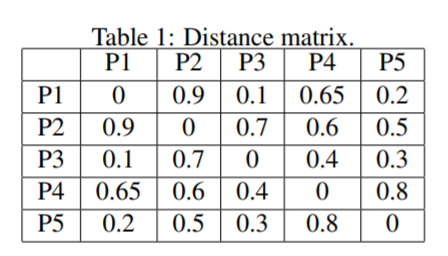
\includegraphics[scale=0.7]{resources/table1.PNG}
        \end{center}
    \end{figure}
    

    \textbf{Solution}\\
    1) Merge P1 \& P3 (0.1)\\
    \begin{table}[H]
        \begin{center}    
        \begin{tabular}{|l|l|l|l|l|}
        \hline
               & P1\&P3 & P2  & P4  & P5  \\ \hline
        P1\&P3 & 0      & 0.7 & 0.4 & 0.2 \\ \hline
        P2     & 0.7    & 0   & 0.6 & 0.5 \\ \hline
        P4     & 0.4    & 0.6 & 0   & 0.8 \\ \hline
        P5     & 0.2    & 0.5 & 0.8 & 0   \\ \hline
        \end{tabular}
        \end{center}
    \end{table}
    2) Merge P1/P3 \& P5 (0.2)\\
    \begin{table}[H]
        \begin{center}
        \begin{tabular}{|l|l|l|l|}
        \hline
                 & P1/P3/P5 & P2  & P4  \\ \hline
        P1/P3/P5 & 0        & 0.5 & 0.4 \\ \hline
        P2       & 0.5      & 0   & 0.6 \\ \hline
        P4       & 0.4      & 0.6 & 0   \\ \hline
        \end{tabular}
    \end{center}
    \end{table}
    3) Merge P1/P3/P5 \& P4 (0.4)\\
    \begin{table}[H]
        \begin{center}
        \begin{tabular}{|l|l|l|}
        \hline
                    & P1/P3/P4/P5 & P2  \\ \hline
        P1/P3/P4/P5 & 0           & 0.5 \\ \hline
        P2          & 0.5         & 0   \\ \hline
        \end{tabular}
        \end{center}
    \end{table}
    4) Merge P1/P3/P4/P5 \& P2 (0.5) \\\\
    Therefore, the dendrogram showing the hierarchical clustering is shown below:\\

    \begin{figure}[H]
        \begin{center}
        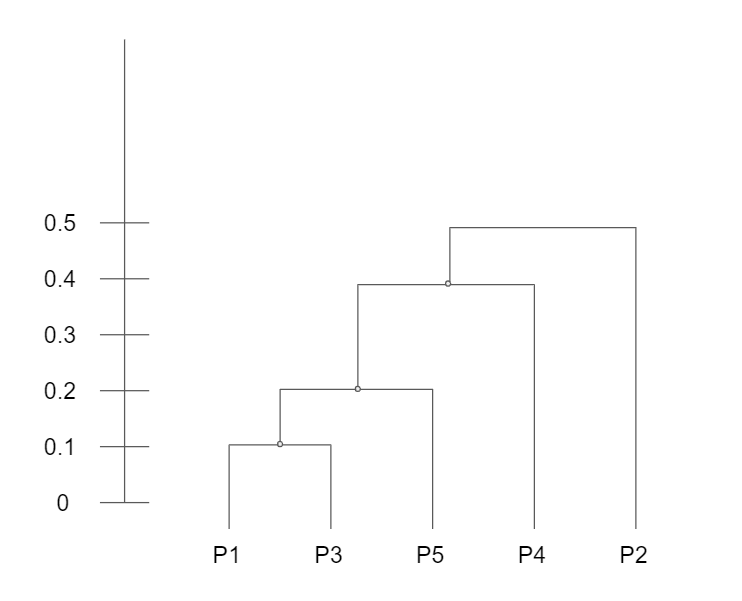
\includegraphics[scale=0.7]{resources/q1.PNG}
        \end{center}
    \end{figure}


\end{homeworkProblem}
\newpage
\begin{homeworkProblem}
    On the 59th page of the lecture notes "Lecture 10", use a dendrogram to show how to perform hierarchical
    clustering with Complete Link on the similarity matrix.

    \begin{figure}[H]
        \begin{center}
        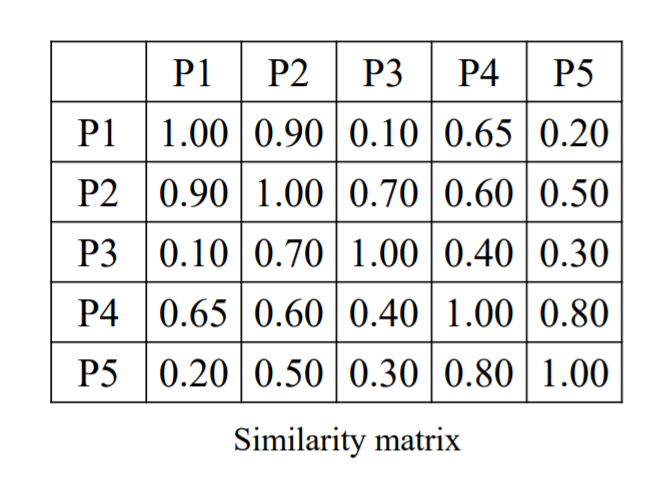
\includegraphics[scale=0.5]{resources/table2.PNG}
        \end{center}
    \end{figure}
    
    \textbf{Solution}\\
    1) Merge P1 \& P2 (0.9)\\
    \begin{table}[H]
        \begin{center}
        \begin{tabular}{|l|l|l|l|l|}
        \hline
               & P1\&P2 & P3  & P4  & P5  \\ \hline
        P1\&P2 & 1      & 0.1 & 0.6 & 0.2 \\ \hline
        P3     & 0.1    & 1   & 0.4 & 0.3 \\ \hline
        P4     & 0.6    & 0.4 & 1   & 0.8 \\ \hline
        P5     & 0.2    & 0.3 & 0.8 & 1   \\ \hline
        \end{tabular}
        \end{center}
    \end{table}
    2) Merge P4 \& P5 (0.8)\\
    \begin{table}[H]
        \begin{center}
        \begin{tabular}{|l|l|l|l|}
        \hline
               & P1\&P2 & P3  & P4\&P5 \\ \hline
        P1\&P2 & 1      & 0.1 & 0.2    \\ \hline
        P3     & 0.1    & 1   & 0.3    \\ \hline
        P4\&P5 & 0.2    & 0.3 & 1      \\ \hline
        \end{tabular}
        \end{center}
    \end{table}
    3) Merge P4/P5 \& P3 (0.3)\\
    \begin{table}[H]
        \begin{center}
        \begin{tabular}{|l|l|l|}
        \hline
                   & P1\&P2 & P3\&P4\&P5 \\ \hline
        P1\&P2     & 1      & 0.1        \\ \hline
        P3\&P4\&P5 & 0.1    & 1          \\ \hline
        \end{tabular}
        \end{center}
    \end{table}
    4) Merge P1/P2 \& P3/P4/P5 (0.1)\\
    Therefore, the dendrogram showing the hierarchical clustering is shown below:\\
    \begin{figure}[H]
        \begin{center}
        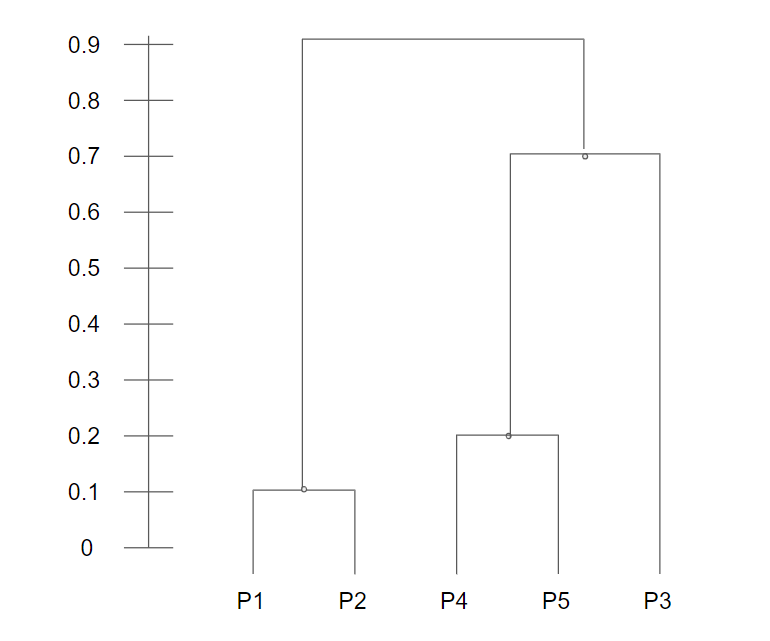
\includegraphics[scale=0.7]{resources/q2.PNG}
        \end{center}
    \end{figure}
    

        

\end{homeworkProblem}



\end{document}